
\chapter{Analýza existujúcich algoritmov pre fuzzifikáciu numerických hodnôt} 

\section{Fuzzy klasifikátor s možnosťou výberu na základe fuzzy entropie} 
Táto sekcia popisuje efektívny fuzzy klasifikátor s možnosťou výberu založenom na meraní fuzzy entropie (FEBFC).
Fuzzy entropia je použitá na vyhodnotenie informácie o distribúcii vzorov v priestore vzorov. S touto informáciou vedia rozdeliť priestor vzorov na disjunktné rozhodovacie oblasti pre rozoznávanie vzorov. Vďaka tomu, že rozhodovacie oblasti sú disjunktné, aj komplexnosť, aj výpočtová náročnosť je zredukovaná. Tým pádom aj čas trénovania a klasifikácie je extrémne krátka. Hoci rozhodovacie oblasti sú rozdelené do disjunktných pod priestorov, môžu dosiahnuť kvalitnú klasifikáciu vďaka tomu, že pod priestory boli správne stanovené navrhovaným meraním fuzzy entropie. Okrem toho sa skúma ďalšie využitie fuzzy entropie na vybraté prvky. Procedúra výberu prvkov nielenže znižuje dimenziu problému, ale aj redukuje šum, zbytočné a nedôležité prvky.

\subsection{Fuzzy entropia na intervale pre každú vlastnosť v rozmere}
FEBFC metóda definuje na základe Shannonovej entropie fuzzy entropiu nasledovne: 
\begin{itemize}
\item[1)] Nech $X={r_1,r_2,\ldots,r_n}$ je univerzálna množina prvkov $r_i$ rozptýlená v vzorkovom priestore, kde   $i=1,2, \ldots, n$. 

\item[2)]
Nech $\tilde{A}$  je fuzzy množina definovaná na intervale vzorkového priestoru, ktorý obsahuje $k$ elementov ($k<n$). Namapovanie stupňa príslušnosti elementu $r_i$
 s fuzzy množinou $\tilde{A}$  sa označuje ako 
$\mu_{\tilde{A}}(r_i)$. 

\item[3)]
Nech $C_1, C_2, \ldots,C_m$  reprezentujú $m$  tried, v ktorých je rozdelených $n$ elementov. 
 
\item[4)]
Nech $S_{C_j}(r_n)$  je množina elementov triedy  $j$  na univerzálnej množine $X$.
Je to podmnožina univerzálnej množiny $X$. 

\item[5)]
Stupeň príslušnosti elementov fuzzy množiny $\tilde{A}$
 triedy $j$ na intervale, kde $j=1,2,\ldots,m$
je defonovaný ako: 
\begin{equation}
{D_j} = \frac{
\sum\limits_{r\in S_{C_j}(r_n)}
\mu_{\tilde{A}}(r)
}{
\sum\limits_{r \in X}
\mu_{\tilde{A}}
\left(r\right)
}. 
\end{equation}

\item[6)]
Fuzzy Entropia $FEC_j(\tilde{A})$ elementov triedy $j$
 na intervale je definovaná ako: 
\begin{equation}\label{eq:eq6}
FEC_j(\tilde{A}) = -D_j \log_2D_j.
\end{equation}
\item[7)]
Fuzzy Entropia $FE(\tilde{A})$ na univerzálnej množine $X$
pre elementy v intervale je definovaná ako: 
$$
FE(\tilde{A}) = \sum\limits FE_{C_j}(\tilde{A}). 
$$

\end{itemize}

 V definícii \ref{eq:eq6} je fuzzy entropia $FEC_j(\tilde{A})$  ako nepravdepodobnostná entropia. Preto môžme zadefinovať nový pojem “stupeň príslušnosti” pre $D_j$. Základná vlastnosť navrhnutej fuzzy entropie je podobná ako Shannonova entropia a spĺňa štyri Luca-Termini axiómy, ale ich spôsob merania informácie je rôzny. Pravdepodobnosť $p_j$ Shannonovej entropie je meraná cez výskyt elementov. Oproti tomu, stupeň príslušnosti $D_j$ v fuzzy entropii je merané príslušenstvom hodnôt vyskytujúcich sa elementov. Okrem toho, fuzzy entropia rozhodovacích oblastiach môže byť získaná cez súčet fuzzy entropie jednotlivých intervalov v každej dimenzii vlastností. 
 
Navrhnutá fuzzy entropia je lepšie schopná rozlíšiť skutočné rozloženie vzorov. Použitím funkcie príslušnosti pre meranie stupňa príšlusnosti, hodnota entropie obsahuje nie len počet vzorov, ale berie aj do úvahy rozloženie vzorov.  
 

\subsection{Operácie fuzzy klasifikátora FEBFC}

V klasifikačnom systéme je najdôležitejší postup rozdelenia priestoru vzoriek do rozhodovacích oblastí. Raz, keď je rozhodovacia oblasť určená, tak sa aplikujú na klasifikáciu neznámych vzorov.  Rozdelenie do rozhodovacích oblastí je súčasťou je súčasťou procesu učenia či tréningového procesu, pokiaľ rozhodovacie oblastí sú rozdelené tréningovými vzormi. 

V fuzzy entropy založeného fuzzy klasifikátora (FEBFC), rozhodovacie oblasti sú uzavreté od povrchov vytváraných z každého rozmeru. Povrchy sú určené rozložením vstupných dát.  
Pri vytváraní intervalov pre každý rozmer, alebo ekvivalentne, sa musí vygenerovať niekoľko trojholníkových funkcií príslušnosti pre každú reálnu hodnotu atribútu (tento proces sa nazýva diskretizácia atribútov). 
Musí byť určený počet intervalov na každom rozmere. Centrum a šírka pre každý interval musí byť vypočítaná. Metóda využíva fuzzy entropiu na určenie vhodného počtu intervalov, a používa k-means algoritmus na určenie stredu intervalov. Potom ako sú určené centrá intervalov je jednoduché rozhodnúť o šírke každého intervalu. 

Z vyššie uvedeného popisu, zhrnúť navrhovanej FEBFC s nasledujúce štyri kroky:
FEBFC sa v stručnosti zrhnúť do týchto štyroch krokov:  
\begin{description}
\item[A.] Určenie počtu intervalov na každý rozmer.
\item[B.] Určenie polohy intervalu, t.j. určenie centra a šírku pre každý interval. 
\item[C.] Priradenie funkcie príslušnosti pre každý interval. 
\item[D.] Označenie tried pre kazdú rozhodovaciu oblasť. 
\end{description}

\subsubsection{A.Určenie počtu intervalov}
Počet intervalov v každom rozmere má zásadný vplyv na určenie účinnosti a presnosti klasifikácie. Ak je počet intervalov príliš veľký, tak bude dlho trvať pokým sa skončí tréningový a klasifikačný proces, a môže nastať pretečenie. 
Na druhú stranu, ak je počet intervalov malý, tak veľkosť každej rozhodovaciej oblasti môže byť veľmi veľká, aby sa zmestila do rozdelenia vstupných vzorov, a výkon klasifikácie sa môže spomaliť. 

Táto časť algoritmu hovorí o tom, ako systematicky zvoliť vhodný počet intervalov. 

Kroky na zvolenie počtu intervalov pre každý rozmer sú nasledovné: 
\begin{description}

\item[Krok 1.] Nastavenie počiatočného počtu intervalov I = 2.
\item[Krok 2.] Nájdenie centier intervalov. 
\item[Krok 3.] Priradenie funkcie príslušnosti pre každý interval. 
\item[Krok 4.] Vypočítanie celkovej fuzzy entropie pre všetky intervaly I a I-1. 
Počíta sa fuzzy entropia na všetkých intervalov, aby sa získala informácia o rozložení vzorov v tejto dimenzii.
\item[Krok 5.] Klesla celková fuzzy entropia? 
V prípade, že celková fuzzy entorpia na intervale I je menšia ako na intervaloch I-1, tak sa znova rozdelia (I = I + 1) a prejde sa na Krok 2, inak sa prejde na Krok 6. 
\item[Krok 6.] I-1 je počet intervalov na zadanom rozmere. 
Vzhľadom na to, že fuzzy entropia neklesá, tak sa zastavilo ďalšie delenie na tejto dimenzii a I-1 je počet intervalov na danom rozmere.   
\end{description}

\subsubsection{B. Určenie polohy intervalov}

Proces určenia polohy intervalov začína s nájdením centrových bodov pre každý interval. Pre nájdenie centier je použitý algorimus CITUJ 36, 37. 
Predpokladajme, že je N počet M-rozmerných vektorov $V_i=(v_{i1}, v_{i2},…, v_{iM} )^T, I = 1, 2, \ldots, N$, čo zodpovedá N elementom. Pre rozdelenie elementov do niekoľkých intervalov v rozmere j, najpr sa extraktuje N hodnot z elementov reprezentujucich tento rozmer $x_i^{(j)} = v_{ij}, i=1, 2, \ldots, N.$ K-means zhlukovací algoritmus je použitý na klasterizáciu $x_i^{(j)} = v_{ij}, i=1, 2, \ldots, N.$

Algoritmus pozostáva z najsledujúcich krokov: 
\begin{description}
\item[Krok 1.] Nastavnie počiatočného počtu zluhov, I. 
\item[Krok 2.] Nastavenie počiatočných stredov klastrov. 
Počiatočné centrá klastrov $c_1, c_2, \ldots, c_I$ môžu byť náhodne vybrané z $x_i^(j) = v_{ij}, i=1, 2, \ldots, N.$ Centrá klustrov $c_q$ ľubovolného klastra q sú priradené nasledovne: 
$$ c_q = \frac{q-1}{I-1}, q = 1, 3, \ldots, I.  $$
\item[Krok 3.] Priradenie označenia klastra pre každý element. 
Po určení klastrových centier,  sa priradí označenie pre každý prvok klastra podľa ktorého stred klastra je najbližšie. Toto je centrum s najmenšou Euclidean vzdialenosťou od prvku. To znamená, že najbližšie centrum spĺňa nasledujúce meranie vzdialenosti: 
$$|{x_i^{(j) – c_q^*}} = min_{1<=q <=I} |{x_i^{(j) – c_q}} $$

Kde $c_q^*$ je najblišie centrum k elementu $x_i^{j}$, teda medzi $c_1, c_2, \ldots,  c_I, c_q^*$ má minimálnu Euclidean vzdialenosť ku $x_i^{(j)}$.

\item[Krok 4.]Prepočítanie klastrových centier. 
Vzhľadom na to, že počiatočné centra sú vybrané náhode, tak sa musí prepočítať  každé centrum nasledujúcim spôsobom: 

 $$c=\frac{\sum\limits_{q=1}^{N_q} x_i^{(j)} }{N_q}, $$
kde $N_q$ je celkový počet vzorov v rovnakom zhluku q. 

\item[Krok 5.] Zmenil sa nejaký cetrum? 
Ak každý klaster center je vhodne určený, prepočítanie centier v kroku 4. to nezmení. Ak áno, zastav určovanie centier intervalov, inak choď na krok 3. 
\end{description}


\subsubsection{C. Priradenie funkcie príslušnosti pre každý interval}

Pridenie funkcie príšlušnosti je procedúra pre priraďovanie funkcie príslušnosti pre každý interval. Na aplikovanie fuzzy entropie sa zhodnotí informácia rozdelenia vzoru v danom intervaly. Priradí sa korešpondujúca funkcia príslusnšosti pre každý interval, aby indikovala stupeň príslušnosti elementu. Hodnota príslušnosti elementu v intervale môže byť videná ako stupeň elementu patriaci tomu intervalu. Intervalový stred má najvyšiu hodnotu príšlušnosti, a hodnota príslušnosti elementu klesá ako vzdialenosť medzi týmito elementami a korešpondujúci interval centra sa zvyšuje.Preto sa priradí najvyšia hodnota príslušnosti 1 centru intervalu, a najnižšia hodnota 0 susedom centra tohto intervalu. V tomto variante sa využíva trojuholníková fuzzy množina. Na obrázku č. \ref{fig:prikladFunkciePrislusnosti} predpokladajme, že $c_1, c_2, c_3, c_4$ sú centrá intervalov. Hodnoty všetkých elementov sú normalizované pre interval [0, 1] pre jednoduchosť. 
Pri priraďovaní funkcie príslušnosti intervalu, tak sa zhodnocujú tieto tri prípady: 

\begin{description}
\item[I. Najľavejší interval] 

V tomto prípade, ako je ukázané na obrázku č. \ref{fig:prikladFunkciePrislusnosti}, prvý centrum intervalu $c_1$ na tomto rozmere ie ohraničený len jedným intervalovým centrom $c_2$. Najvyššia hodnota príslušnosti 1 tohto intervalu sa nachádza v $c_1$, kde je najnižšia hodnota príslušnosti 0 je v $c_2$. Keď $x=0$, hodnota príslušnosti je určená ako 0.5, ako je ukázané na obrázku č. \ref{fig:prikladFunkciePrislusnosti}. Funkcia príslušnosti $\mu_{i1}$ najľavejšieho intervalu na rozmere i je definovaná nasledovne:  

$$
\mu_{i, 1}(x) = 
\begin{cases}
{\frac{c_1 + x}{2c_1}, } &  \textrm{pre } x \leq   c_1 ,
\\
\textrm{max} \left\{1 -\frac{| x-c_1|}{ | c_2 - c_1 |} \right\},
&  \textrm{pre } x >  c_1, \end{cases}
$$

kde $c_1$ je centrum najľavejšieho intervalu, a $c_2$ je centrum prvého centra intervalu vpravo od $c_1$. 

\item[II. Najpravejší interval ]
V tomto prípade, ako je ukázané na obrázku  č. \ref{fig:prikladFunkciePrislusnosti}, funkcia príslušnosti $\mu_{i4}$ najpravejšieho intervalu na rozmere i je definovaný nasledovne:

\begin{displaymath}
\mu_{i, 4}(x) = 
\begin{cases} 
\textrm{max} \left\{
1 -\frac{| c_4-x|}{c_4-c_3} , 0
\right\}, 
& \textrm{pre } x \leq   c_4 ,
\\ 
\frac{2- x - c_4 }{2(1-c_4)}, 
& \textrm{pre } x >   c_4 ,
  \end{cases}, 
\end{displaymath}

kde $c_4$ je centrom najpravejšieho intervalu, a $c_3$ je centrom prvého intervalu vľavo od $c_4$. 


\item[III. Interný interval]
V tomto prípade, ako je ukázané na obrázku  č. \ref{fig:prikladFunkciePrislusnosti}, center $c_3$ interného intervalu je ohraničený jeho ľavým intervalovým centrom $c_2$ a pravým intervalovým centrom $c_4$. Najvyšia hodnota príslušnosti sa nachádza v $c_3$, a najnižšie honoty sú v centrách $c_2$ a $c_4$. Funkcia príslušnosti $\mu_{i3}$ je tretím intervalom v rozmere \textit{i} v tomto prípade definovanom ako  
$$
\mu_{i, 3}(x) = 
\begin{cases}
\textrm{max} \left\{
1 -\frac{| c_3-x|}{|c_3-c_2|} , 0
\right\}, 
& \textrm{pre } x \leq   c_3,
\\
\textrm{max} \left\{
1 -\frac{| c_3-x|}{|c_4-c_3|} , 0
\right\}, 
& \textrm{pre } x >  c_3.
\end{cases} 
$$

\end{description}

\begin{figure}[h]
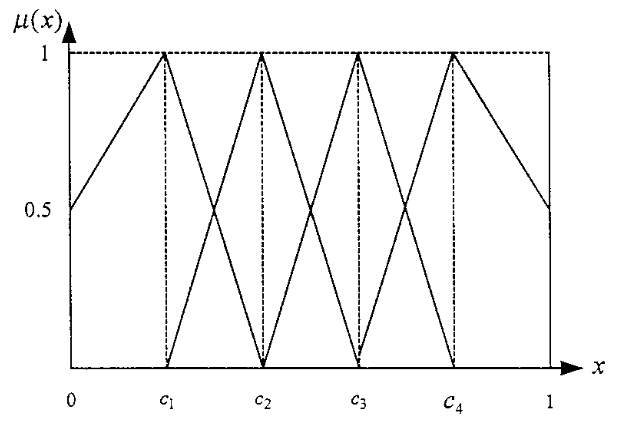
\includegraphics[width=0.75\textwidth]{obrazky/prikladFunkciePrislusnosti4}
\centering
\caption{Príklad priradenia funkcie príslušnosti pre intervalové centrá $c_1, c_2, c_3, c_4$ a trojuholníky korešpondujúce s funkciou príslušnosti. \cite{TODO}} 
\label{fig:prikladFunkciePrislusnosti}
\end{figure}

\subsubsection{D. Označenie tried pre každú rozhodovaciu oblasť}
Pre určenie označení tried pre každú rozhodovaciu oblasť sa musí použiť metóda na určenie fuzzy entropie. Fuzzy entropia rozhodovacích oblastí pre vzory každej triedy sú počítané, aby sa určila trieda pre každú rozhodovaciu oblasť.Fuzzy entropia rozhodovacích oblastí môže byť získaná cez sumarizáciu fuzzy entropie individuálnych intervalov pre každú vlastnosť rozmeru. Triede sa priradia rozhodovacia oblasť s najnižšou fuzzy entropiou v tejto oblasti.  Raz keď je rozhodovacia oblasť priradená a trieda označená, tak trénovaci proces je kompletný. 

\subsection{Výber vlastností}
Nový prístup pre výber funkcie založenej na fuzzy entropii je popísaný v nasledujúcom odseku. Fuzzy entropia odráža viac informácií v aktuálnom rozložení vzorov v priestore vzoriek. Vzhľadom k tomu, že fuzzy entorpia je schopná rozlíšiť rozdelenie vzorov lepšie, používa sa na hodnotenie oddeliteľnosti jednotlivých funkcií. 

Intuitívne, keď je nižšia fuzzy entropia vlastností, tak tým vyššia je diskriminácia vlastností. Procedúra na výpočet fuzzy entropie pre každú vlastnosť je opísaná nasledovne: 
\begin{itemize}
\item [Krok 1.] Určenie počtu intervalov. 
\item [Krok 2.] Určenie polohy intervalov. 
\item [Krok 3.] Priradenie funkcie príslušnosti pre každý interval. 
\item[Krok 4.] Vypočítanie fuzzy entropie pre každú vlastnosť cez sumarizáciu fuzzy entropie vo všetkých intervalov v tomto rozmere vlastnosti.  
\end{itemize}

Potom, čo bola určená fuzzy entropia pre každú vlasnosť, tak sa môžu vyberať vlastností podľa výberu dopredu (\textit{forward selection}) alebo dozadu \textit{backward elimination}. Metóda výberu dopredu je určenie relavantných vlastností na začiaktku s práznou množinou a iteratívne pridávať vlastností pokým sú splnené kritérium na zastavenie. Na rozdiel od toho eliminačná metóda vzad začína so všetkými vlastnosťami v množine, a odstraňuje vlastností pokým sú splnené kritérium na zastavenie.  
V FEBFC procese sa používa eliminačná metóda vzad na selektovanie relavantných vlastností a kritérium zastavenia v tejto metóde je založená na klasifikácii rýchlosti triedičia.  Vzhľadom k tomu, že vlastností s vyššou fuzzy entropiou sú málo relavantné pre klasifikačný cieľ, tak sa odstránia vlastnosti ktoré majú najvyššiu fuzzy entropiu, ak to neznži mieru klasifikácie. Potom sa opakuje vyššie spomenutý krok až pokým všeký irrelavantné vlasností sú odstránené. Napokon, ľavé vlastností sú určené ako vlastností pre klasifikáciu. 
S touto selekciou vlastností sa môže znížiť problém s rozmerom, aby sa urýchlil proces klasifikácie. V niektorých prípadoch sa môžu dosianúť lepšie výsledky klasifikácie tým, že odhalíme nadbytočné, šumivé alebo nedôležité vlastnosti. 

\subsubsection{Záver FEBFC metódy}
Cieľom tradičnej klasifikácie vzorov je rozdelenie priestoru vzoriek do rozhodovacích oblastí, jednu oblasť pre každú triedu. V mnotých klasifikačných systémoch, rozhodovacie oblasti sú rozdelené do prekrývajúcich sa oblastí. Hoci klasifikátor s prekrývajúcimi rozhodovacími oblastiami môže dosiahnúť lepšiu klasifikačnú výkonnosť, ale to trvá dlhšie pre uzatvorenie rozhodovacích oblastí. 

Táto metóda je prezentovaná ako efektívny klasifikátor s výberom vlastností založený na fuzzy entropii pre klasifikáciu vzoru. Vzorový priestor je rozdelený do neprekrývajúcich fuzzy rozhodovacích oblastí. Vzhľadom na to, že rozhodovacie oblastí sú fuzzy podoblasti, tak sa môžu získať hladké hranice, pre dosiahnutie lepšieho výkonu klasifikácie. Aj keď rozhodovacie oblastí sa neprekrývajú, tak môžu znížiť výpočtovú zložitosť a záťaž klasifikátora.  

Tiež sa používa fuzzy entropia na vybranie relavantných vlastností. Aplikovanie výberu vlastností nielen zníži problém s rozmerom, ale ako aj zlepší výkonnosť klasifikácie odstránenim zbytočných, šumivých, nedôležitých vlastností. Taktiež algoritmus K-means zhlukovania bol použitý na určenie funkcie príslušnosti pre každú vlasnosť. 



\section{Fuzzy klasifikátor založený na hierarchickej fuzzy entropii}

Fuzzy klasifikátor založený na hierarchickej fuzzy entropii (FC-HFE) je algoritmus, ktorý vychádza z algoritmu fuzzy klasifikátora s možnostou výberu na základe fuzzy entropie (FEBFC). 

Metóda FEBFC má nasledovné problémy: 
\begin{itemize}
\item Označovanie tried pre každú rozhodovaciu oblasť je vykonávané podľa fuzzy entropy sumácie pre individuálne intervaly pre každú dimensiu. Rozhodovacia oblasť je priradená triede s najnižšou fuzzy entropiou v danej oblasti. Podľa axiómu fuzzy entropie, fuzzy entropia bude nula, či zhodovací stupeň pre každú triedu je nula alebo jedna. Preto, priraďovanie tried bude mať chyby, keď počet tried v ktorých fuzzy entropia sa rovna nule je viac ako jeden v tejto oblasti. 

\item V FEBFC, rastúci počet intervalou na každej dimensii je vykonaný podľa pravidla, ktoré celkovú entropiu I (počet intervalov v špecifickej dimenzii) intervalov je menej ako to pre I-1 intervalov. Toto pravidlo niekedy zabraňuje v raste počtu intervalov, ktoré vedie k nesprávnej klasifikácii. Napríklad, dáta sú prezentované ako even intersecting distribution, ako spiral dáta.  Fuzzy entropia spiral data typu je na začiatku vysoká, dáta by mali byť neskôr rozdelené na základe klesajúcej fuzzy entropie. Preto zastavujúca podmienka algoritmu pre rastúci počet intervalov bude výsledok v obmedzení rastúceho počtu intervalov na každej dimenzii. 

\item Vzorový priestor bol rozdelený do neprekrývajúcich sa rozhodovacích oblastí použitím mriežkového rozdelenia. Označovanie tried nemôže byť priradené do rozhodovacej oblasti, ktorá nemá žiadne trénovacie dáta. Ak testovacia vzorka padá do danej rozhodovaciej oblasti, ktoré systém nevie ako klasifikovať. 
\end{itemize}

FC-HFE upravuje pôvodnú metódu FEBFC v určovaní počtu intervalov najpr. FC-HFE udržiava pôvodnu podmienku pre zastavenie rastu počtu intervalov, keď celková entropia I intervalov je viac ako jeden z I-1 intervalu. Ďalšia podmienka pre zastavenie rastu počtu intevalov, je ak celková fuzzy entropia I intervalov je viac ako jedna z I-1 intevalu a celková fuzzy entropia I-1 intervalov je menej ako prahová hodnota  $\varphi$ $($ to je, keď celková fuzzy entropia I intervalov je menšia ako jedna z I-1 intervalu alebo celková entropia I intervalu je viac ako prahová hodnota $\varphi$, tak $I=I+1)$. Hodnota prahovej hodnoty $\varphi$ bola obdržaná použítím nasledovnej rovnice:$$\varphi= -N_{trieda}\cdot \frac{1}{N_{trieda}} \cdot \log_2{(\frac{1}{N_{trieda}})}\cdot (I-1) \cdot \theta = - \log_2{(\frac{1}{N_{trieda}})}\cdot(I-1)\cdot\theta$$
kde $N_{trieda}$ je počet data tried, a $\theta$ je percento maximálnej celkovej fuzzy entropie z I-1 intervalov. $\theta$ môže byť ladený použitím odlišného klasifikačného problému. Preto, môžu produkovať dostatok intervalov pre rovnomerné preniky dáta distribúcii použitím tejto metódy. Fuzzy entorpia pre každú dimensiu musí byť menej ako špecifická hodnota. 

Ďalší fenomén, ktorý sa našiel v FEBFC je hodnota fuzzy entropie pre niektoré rozhodovacie oblasti je vždy veľmi vysoká (to je data distribúcia rozhodujúcej oblasti je veľmi zmätená alebo dáta, ktoré sú klasifikované nesprávne je veľmi veľa) snáď vzorkový priestor je rozdenený do toľko rozhodovacích oblastí fuzzy entropiou, zabraňujúc narastaniu klasifikačnej hodnote. 

FC-HFE  metóda sa zaoberá vyšou fuzzy entropiou rozhodovacích oblastí nazývaních hierarchická fuzzy entorpia. Štruktúra je zobrazená na obrázku TODO OBRAZOK X. 2D vzorkový priestor na Obr.1 je rozdelený do nerovnomerných 53 rozhodovacích oblastí hierarchickou fuzzy entropiou. Prvá až štvrtá rozhodovacia oblasť fuzzy entropie vrstvy I je veľmi vysoká. Rozdelili tieto rozhodovacie oblasti. Nparíklad rozhodovacia oblasť I bola rozdelená do ôsmych rozhodovacích oblastí po druhý raz. Rozhodovacie podoblasti I a II boli rozdelené do štyroch rozhodovacích oblastí retrospektívne po tretí raz. Rozhodovacie oblasti I boli rozdelene do štrnástich rozhodovacích oblastí. Fuzzy entorpia väčšiny rozhodovacích oblastí sa stala nižšou po tom, ako bol vzorkový priestor rozdelený použitím hierarchickej fuzzy entropie. 

Okrem toho, FC-HFE modifikoval metódu, ktorou sa počíta fuzzy entorpia pre rozhodovacie oblasti. Ak tam nie sú žiadne trénovacie dáta určitej triedy na intervale, a tak množina fuzzy entropie tejto triedy sa rovná jednej, aby sa zabránilo tomu, že fuzzy entorpia určitej triedy sa bude rovnať nule viac ako jeden pre počítanie najnižšiej fuzzy entorpie oblasti. 

{Algorimtus klasifikácie – Fuzzy klasifikátor založený na hierarchickej fuzzy entropii (FC-HFE)} má nasledujúce kroky. 

\textbf{Krok 1 – Krok 4.} je rovnaký ako FEBFC v selektovaní počtu intervalov pre každú dimenziu na aktuálnom vzorovom priestore. 

\textbf{Krok 5.} Ak celková fuzzy entropia I intervalu je menej ako I-1 intervalu alebo celkova fuzzy entropia I intervalu je viac ako prahova hodnota $\varphi$, tak sa znova rozdeluje $(I = I - 1)$ a ide na krok 2. Inak sa zastavi zvyšovanie intervalov na tejto dimenzii a rozhodne sa počet intervalov pre ďalšiu dimenziu. 

\textbf{Krok 6.} Akonáhle intervaly pre každú dimeziu sú určené, rozhodovacie oblasti pre súčasný vzorkový priestor sú rodelené. Mean fuzzy entropie je vypočítaní použitím nasledujúcej rovnice pre všetky rozhodovacie oblasti: 
$$MFE_i =  \frac{\sum\limits_{i=1}^{N_i}FE_{ij}}{ N_i},  j=1…N_i$$
Kde $N_j$ je počet rozhodovacích oblastí pre i-tú vrstvu, $FE_{ij}$ je j-tá rozhodovacia oblasť pre i-tú vrstu a $MFE_i$ je mean fuzy entropy pre i-tú vrstvu. 

\textbf{Krok 7.} Fuzzy entropy pre každú rozhodovaciu oblasť v súčasnom vzorovom priestore je porovnávaný s MFE. Ak fuzzy entorpia pre rozhodovaciu oblasť je vačšia ako mean fuzzy entropie, oblasť sa stane nezávislým podpriestorom a krok 1. až krok 7. sú vykonávané znova na determinovanie rozhodovacích oblastí pre každy podpriestor. Inak rozhodovacia oblasť bude pridelená označeniu triedy. 

Horeuvedený proces je ako rekurzívna funkcia, ktorá je vykonávaná opakovane pre každý podpriestor pokiaľ všetky podpriestory nemôžu byť viac rozdelené. Keď horné kroky sú skončené, testovací vzor je klasifikovaní použitím rozhodovacích oblasti, ktorá majú označenie triedy. Keď testovacia vzorka nemá označenie triedy oblasti triedy, tak testovacia vzorka ej porovnávaná použitím krátkej Euclidovej vzdialenosti medzi susemi trénovacích dát a testovaciej vzorky, klasifikované do najbližšej trénovacej triedy. 




\section{Fuzzy k-means (FCM) algoritmus}
%https://www.mathworks.com/help/pdf_

%doc/fuzzy/fuzzy.pdf
Fuzzy k-means (FCM) je metóda, ktorá umožňuje zhlukovanie pre každý dátovy bod, ktorý môže patriť do viacerým klastrov s rôznym stupňami príslušnosti. 
\cite{Bezdec1981}

FCM je založená na minimalizácii účelovej funkcie\cite{fuzzyLogicToolbox}

$$J_m = \sum_{i=1}^{D}\sum_{j=1}^{N} { \mu_{ij}^m \left| \left| x_i - c_j \right|\right|^2  },$$ 
kde 
D je počet dátových bodov, N je počet klastrov, m je fuzzy časť exponentu matice pre riadenie stupňa fuzzy prekrytia,  m $>$ 1. 
Fuzzy prekrytie určuje ako rozmanité hranice sú medzi klastrami a aký počet dátových bodov majú významnú príslušnosť vo viac ako v jednom klastri. 
%fuzzy partition matrix exponent for controlling the degree of fuzzy overlap, with m > 1. 
Ďalej $x_i$ je i-tý dátový bod,  $c_j$ je centrum j-tého klastra, $\mu_{ij}$ je stupeň príslušnosti $x_i$ v j-tom klastri. 
 
Kroky Fuzzy k-means algoritmu : 
\paragraph{Krok 1.} Náhodne sa inicializuje kluster hodnoty príslušnosti, $/mu_{ij}$. 
\paragraph{Krok 2.} Vypočítanie centier klastra
$c_j = \frac{
\sum\limits_D^{i=1} \mu_{ij}^m x_i 
}{
\sum\limits_D^{i=1} \mu_{ij}^m
}$

\paragraph{Krok 3.} Aktuálizácia $\mu_{ij}$ podľa nasledujúceho vzťahu  
$\mu_{ij} = \frac{1}{\sum\limits_{k=1}^N  \left ( \frac {\left| \left| x_i - c_j \right|\right|}{\left| \left| x_i -c_k\right|\right|}\right) ^{\frac{2}{m-1}}}. $


\paragraph{Krok 4.} Vypočítanie účelovej funkcie $J_m$. 
\paragraph{Krok 5.} Opakovanie krokov 2-4 až pokým $J_m$ sa zlepší o menej než stanovená minimálna prahová hodnota alebo po uplynutí určitého maximálneho počtu iterácií. 





\section{Viacintervalová diskretizácia spojitých hodnotových atribútov pre klasifikačné učenie}

V tejto metóde je použitá heuristická minimalizácia entropie pre diskretizáciu v spojitom rozsahu do viacintervalového. 

\subsection{Minimálny opis dĺžkového princípu }

Minimálny opis dĺžkového princípu (MDLP) objektu je difinovaný ako minimálne číslo bitov potrebné na jedinečné určenie toho či objekt bude odstránený z množiny objektov. 
MDLP je všeobecný princíp, ktorý je určený na kódovanie prirodeného stavu vo vede smerom k jednoduchším teóriám, ktoré vysvetlia rovnaké telo dát. 

TODO


\section{Modifikovaný MDLP}	

find and correct a program that samples the data (attributes) in accordance with the criterion of MDLP (minimum description length partition), based on entropy and having built a stopping criterion.

1. MDLP method developed in the
Fayyad, U. M. and Irani, K. B. (1993). Multi-interval discretization of continuous-valued attributes for classification learning, Artificial intelligence, 13, 1022-1027.
I had an interactive version of the program, which lets you choose from several stopping criteria:
1) using the criteria proposed in the original work;
2) criteria for the number of partitions intevalov;
3) criteria for the threshold Gini index (which assesses the effectiveness of the partition at the point in terms of the decrease in entropy).
TODO = TOTO JE TEN RUSOV ALGORITMUS

\subsection{Algoritmus MDLP}
todo 




























\section{Modifikovaný FEBFC algoritmus cez váženú entropiu }

Modifikácia algoritmu je v spôsobe výpočtu funkcie príslušnosti lingvistickej premennej, tak aby hodnota sumy hodnôt funkcie príslušnosti bola rovná 1. Ďalej pri výbere kritéria efektívnosti rozkladu na intervaly v tvare váženej fuzzy entorpie, ktorá berie do úvahy aj počet elementov patriacich do získaných intervalov. \cite{levashenkoProj}

Základná myšlienka spočíva v postupnom rozklade množiny $X$ na $2,\ldots, n$ intervalov a kontrole efektívnosti tohto rozkladu. 


\subsection{Algoritmus transformácie reálnych hodnôt na lingvistickú premenú }

\subsubsection{Vstupné dáta}
Počet N hodnôt vstupného atribútu, zadaného množinou reálnych čísel $X={x_1, \ldots,x_i, \ldots, x_N}$. 
Počet K možných hodnôt výstupného atribútu $B={b_1, \ldots, b_k, \ldots, b_K}$, ku ktorým patria prvky množiny X. Množina dvojíc $(x_i b_k)$ definuje  vzťah medzi každou hodnotou množiny X a hodnotou výstupného atribútu. \cite{levashenkoProj}

\subsubsection{Výstupné dáta}
Počet Q intervalov, na ktoré je potrebné rozložiť vstupnú množinu reálnyc čísel X (počet termov lingvistickej premennej). Matica príslušnosti U s rozmermi $N \times Q$. \cite{levashenkoProj}

\subsubsection{Kroky algoritmu}
Algorimtus sa skladá z ôsmych krokov. 

\begin{itemize}
\item[]{Krok 1.}   Určenie počiatočného počtu intervalov Q = 2. 
\item[]{Krok 2.} Vybratie počiatočného centra každého intervalu $\left\{C_1, \ldots, C_Q\right\}$. 

Výber centra je realizovaný 
	\begin{itemize}
	\item náhodným výberom hodnôt spomedzi čísel $x_i$ alebo 
    \item rovnomerným rozkladom množiny všetkých hodnôt na Q intervalov 
    $$C_q=\frac{q-1}{Q-1},$$ kde $q=1,\ldots, Q. $
	\end{itemize}
    
 \item[]{Krok 3.}  Určenie intervalu, kde patrí každý element $x_i$. Kritérim príslušnosti je najmenšia hodnota euklidovskej vzdialenosti, alebo iná vzdialenosť tohto elemntu $x_i$ a centier všetkých intervalov $\left\{C_1, \ldots, C_Q\right\}$ , kde interval 
 $$q_{\min}=\min_{q=1, \ldots, Q} |x_1 - C_q|. $$
 
  \item[]{Krok 4.}
  Nové centrá sú určené pre každý interval $\left\{C_1, \ldots, C_Q\right\}$ ako aritmetický priemer hodnôt prvkov $x_i$, patriacich do týchto intervalov
  $$
  C_q = \frac{1}{N_q} \times \sum\limits_{i=1}^{N_q} x_i , 
  $$
  kde $N_q$ je počet prvkov $x_i$ patriacich do intervalu $C_q$. 
  
  
  
   \item[]{Krok 5.} Ak sa jedno z vypočítaných nových centrier zmenilo, tak sa pokračuje krokom 3, v opačnom prípade krokom 6. 
   
   
    \item[]{Krok 6.} Definícia funkcii príslušnosti lingvistickej premennej pre každý z Q termov. Získaný výsledok predstavuje hľadanú maticu príslušnosti \textbf{U}. 
    Pre najľavejší interval je definovaná funkcia príslušnosti nasledovne  
    $$\mu_{A_1}(x_i) = 
\begin{cases}
1 & x_i \leq  C_1,
\\
\frac{C_2-x_i}{C_2-C_1} & C_1 < x_i < C_2, 
\\
0 & x_i > 0.
\end{cases}$$

Pre krajový pravý interval je definovaná funkcia príslušnosti nasledovne 
    $$\mu_{A_1}(x_i) = 
\begin{cases}
0 & x_i \leq  C_{Q-1},
\\
\frac{x_i-C_Q}{C_Q-C_{Q-1}} & C_{Q-1} < x_i < C_Q, 
\\
1 & x_i \geq C_Q. 
\end{cases}$$

Pre vnútorný interval je definovaná funkcia príslušnosti nasledovne 
$$\mu_{A_1}(x_i) = 
\begin{cases}
0 & x_i \leq  C_{Q-1},
\\
\frac{x_i-C_{q-q}}{C_q-C_{q-1}} & C_{q-1} < x_i < C_q, 
\\
\frac{C_{q+1}-x_i}{C_{q+1}-C_q} 
& C_q < x_i \leq C_{q+1},
\\0 & x_i >  C_{Q+1}.
\end{cases}
    $$
 
\item[]{Krok 7.} 
 Vypočítanie váženej fuzzy entropie $wFE(A)_Q$ pri rozklade na Q intervalov. 
 
 \item[]{Krok 8.} 
 Porovanie vypočítanej fuzzy entropie $wFE(A)_Q$ s predošlou hodnotou $wFE(A)_{Q-1}$, pričom hodnota $wFE(A)_1$ je veľké číslo ($+\infty$). 
 V prípade, že táto entropia neklesá, tak sa zväčší počet intervalov $Q=Q+1$ a zopakujú sa všetky výpočty vrátane kroku 2. 
 V opačnom prípade hodnota $(Q-1)$ je optimálny počet intervalov. 
\end{itemize}












